\chapter{Twierdzenie Ramseya}
Twierdzenie Ramseya mówi o konieczności pojawienia się pewnych układów w pozornym chaosie\cite{dickson}, co oznacza że każda większa struktura będzie zawierała jakąś podstrukturę. Zagadnienie można łatwo przedstawić posługując się teorią grafów, dla uproszczenia zostanie użyte kolorowanie dwoma kolorami.

\begin{theorem}
Niech $r \in \mathbb{N}$. Istnieje takie $n \in \mathbb{N}$  gdzie dla każdego 2-kolorowego $\mathit{K}_{n}$ grafu znajdzie się jednokolorowy podgraf $\mathit{K}_{r}$ w $\mathit{K}_{n}$.  \cite{theory} 
\end{theorem}

Na potrzeby pracy będziemy omawiać tylko dwukolorowe struktury. W celu ułatwienia obliczeń i umożliwienia użycia technik generacji grafów, używamy uproszczenia reprezentacji grafowej. Zamiast wyznaczać kolorowania grafu pełnego, używamy wszystkich grafów prostych gdzie kolor krawędzi zamieniony jest na istnienie lub brak istnienia krawędzi pomiędzy parą wierzchołków.

\begin{definition}[Liczba Ramseya]
Niech $r \in \mathbb{N}$ i $b \in \mathbb{N}$. Liczba Ramseya, wyrażana jako $n = R(r,b)$, jest najmniejszą liczbą całkowitą taką że każdy $n$-wierzchołkowy graf będzie zawierał klikę rzędu $r$ lub zbiór niezależny rzędu $b$.
  \cite{mainpaper} 
  \label{lram}
\end{definition}

Definicje \ref{lram} inaczej można wyrazić posłując się kolorowaniem grafów, gdzie $n$ jest najmniejszą liczbą całkowitą, która określa rozmiar kliki w której musi powstać czerwony monochromatyczny podgraf $\mathit{K}_{r}$ lub niebieski monochromatyczny podgraf $\mathit{K}_{b}$

\begin{definition}[Graf Ramseyowski]
Niech $r \in \mathbb{N}$, $b \in \mathbb{N}$ i $n \in \mathbb{N}$. Graf Ramseyowski, zapisany jako $R(r,b,n)$ oznacza graf mający $n$ wierzchołków, nie zawierający kliki o rozmiarze $r$ i nie zawierający zbioru niezależnego rozmiaru $b$.  \cite{mainpaper} 
\label{gram}
\end{definition}

Oznacza to, że graf spełniający R(4,5,6) to graf zbudowany na 6 wierzchołkach, który nie posiada kliki 4 rzędu ani zbioru niezależnego 5 rzędu. Przykładowy graf R(4,5,6) jest przedstawiony na rysunku \ref{pgram}

 \begin{figure}[H]
  \centering
   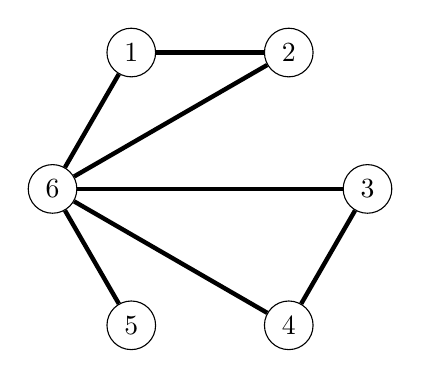
\begin{tikzpicture}[node distance={15mm}, main/.style = {draw, circle}] 
 \node[main] (3) at (0:2) {$3$};
 \node[main] (2) at (60:2) {$2$};
 \node[main] (1) at (120:2) {$1$};
 \node[main] (6) at (180:2) {$6$};
 \node[main] (5) at (240:2) {$5$};
 \node[main] (4) at (300:2) {$4$};

\draw[ultra thick] (6) -- (1);
\draw[ultra thick] (6) -- (2);
\draw[ultra thick] (6) -- (3);
\draw[ultra thick] (6) -- (4);
\draw[ultra thick] (6) -- (5);
\draw[ultra thick] (3) -- (4);
\draw[ultra thick] (2) -- (1);
    \end{tikzpicture}
    \caption{}
    \label{pgram}
 \end{figure}

Celem tej pracy jest wykazanie, że stworzenie grafu $R(4,5,25)$ jest niemożliwe, a istnieją grafy $R(4,5,24)$, z czego wynika, że liczba Ramseya $R(4,5) = 25$.


\section{Historia liczby i twierdzenia Ramseya}

W 1930 roku zostało opublikowane dzieło Franka Plumptona Ramseya ''On a Problem of Formal Logic''\cite{ramsey} , które posłużyło jako podstawę do teorii którą dzisiaj znamy jak Teoria Ramseya. 


\subsection{Twierdzenie Van der Waerden's}
Twierdzenie opublikowane przez Van der Waerdena w 1927 roku, przed powstaniem Twierdzenia Ramseya lecz uważana za jedną z jego gałęzi. 

\begin{theorem}
Dla dowolnych liczb naturalnych $r$ oraz $k$ istnieje taka liczba naturalna $n$ która określa zbiór \{1, 2, 3, ..., $n$\} który jest pokolorowany na $r$ różnych kolorów, z $k$ liczbami naturalnymi w ciągu arytmetycznym, które są tego samego koloru.\cite{theory} 
\end{theorem}

Dla przykładu, $W(2,3) = 9$. Zbiór o ośmiu elementach można podzielić na następujące podzbiory aby w żadnym z podzbiorów nie wystąpił szereg arytmetyczny o trzech elementach, \{1,2,3,4,5,6,7,8\} $\to$ \textcolor{red}{\{1,2,5,6\}},\textcolor{blue}{\{3,4,7,8\}}. W przypadku zbioru o dziewięciu elementach taki podział nie jest możliwy. Dodając 9 do dowolnego podzbioru utworzony zostanie ciąg arytmetyczny o trzech elementach np. \textcolor{red}{\{1,5,9\}} lub \textcolor{blue}{\{7,8,9\}}. Podobna sytuacja zajdzie dla podziału \textcolor{red}{\{1,4,5,8\}},\textcolor{blue}{\{2,3,6,7\}}.

\subsection{Paul Erd\"os i teoria Ramseya}

\begin{definition}[Pozycja ogólna]
 Układ punktów, gdzie żadne trzy punkty nie są współliniowe. \cite{gpos}
\end{definition}

Happy Ending problem, czyli problem zaprezentowany przez Paula Erd\"osa oraz Georga Szekeresa w 1933 roku brzmi następująco. 

\begin{theorem}
Dla dowolnej liczby całkowitej N, istnieje taka liczba punktów w przestrzeni, w pozycji ogólnej, która zawiera podzbiór składający się z N punktów, który tworzy wielokąt wypukły.
 \cite{erdoshappy} 
\end{theorem}

Prace nad Happy Ending problem sprawiły, że Paul Erd\"os natrafił na publikacje Ramseya z 1930 roku\cite{theory}. Spowodowało to że Erd\"os rozpoczął prace nad liczbami Ramseya, co przyczyniło się do rozwoju tej teorii.


\hfill  \par
Party problem lub inaczej Theorem on Friends and Strangers, jest to problem dzięki któremu można przedstawić przykład zastosowania liczby Ramseya. Brzmi on następująco: jaka jest najmniejsza liczba osób jaką trzeba zaprosić na przyjęcie tak aby trójka z nich były wspólnymi znajomymi lub trójka z nich była dla siebie nieznajomymi\cite{partyproblem}? Aby odpowiedzieć na to pytanie można skorzystać z teorii Ramseya, gdzie znajdziemy, że odpowiedź na postawione pytanie stanowi liczba Ramseya $R(3,3)=6$, która jest opisana w dalszej części pracy. Powyższe pytanie można przedstawić w bardziej formalny sposób: 
\begin{itemize}
\item Znajdź najmniejszą liczbę gości, którzy muszą zostać zaproszeni tak aby przynajmniej $m$ znało się wzajemnie a $n$ była dla siebie obca \cite{partyformal}
\item Znajdź najmniejszą liczbę wierzchołków dla których graf będzie zawierać klikę stopnia $n$ lub zbiór niezależny stopnia $m$.
\end{itemize}
Rozwiązaniem dla tego problemu są liczby Ramseya. 

\section{Wartości liczb Ramseya}

%\begin{enumerate}  

%  \item $R(1,k)$ = $R(k,1)$ = 1 \hfill \par
 Rozważmy $R(1,k)$ = $R(k,1)$ = 1.  W przypadku gdy jeden z parametrów wynosi 1 aby spełnić warunek wystarczy jeden wierzchołek.  Jednokolorowy graf $\mathit{K}_{1}$ jest pojedynczym wierzchołkiem i spełnia zarówno warunek dla $R(1,b)$ oraz $R(r,1)$, patrz rysunek \ref{grafk1}. 
  
  \begin{figure}[h]
  \centering
  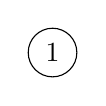
\begin{tikzpicture}[node distance={15mm}, main/.style = {draw, circle}] 
    \node[main] (1)  {$1$};

   \end{tikzpicture}
   \caption{R(1,k,1)}
   \label{grafk1}
\end{figure}
  
  \hfill \par
%   \item $R(2,k)$ = $R(k,2)$ = $k$ \hfill \par
	Rozważmy $R(2,k)$ = $R(k,2)$ = $k$. W przypadku gdy jeden z parametrów wynosi 2 nie możemy postąpić analogicznie jak w przypadku gdy $k$=1, gdyż graf $\mathit{K}_{2}$ nie spełni warunku gdy $k$ > 2 dla kolorowania jednym kolorem. Tak samo każdy graf pełny o rozmiarze mniejszym niż $k$ nie spełnia warunku w sytuacji gdy zostanie użyty kolor ograniczony liczbą $k$ aby pokolorować go w jednolity sposób. Dlatego też liczba wierzchołków w grafie musi wynosić k co zawsze spełni jeden z dwóch warunków, pierwszy w przypadku, gdy wszystkie krawędzie zostaną pokolorowane jednym kolorem lub drugi, gdy chociaż jedna krawędź będzie drugiego koloru. Przykładowo dla $R(2,4)$ gdzie pierwszy kolor (dla $r$=2) będzie oznaczony kolorem czerwonym a drugi ($b$=4) niebieskim, patrz rysunek \ref{grafk2}.
	
\begin{figure}[H]
  \centering
  \subfloat[]{
   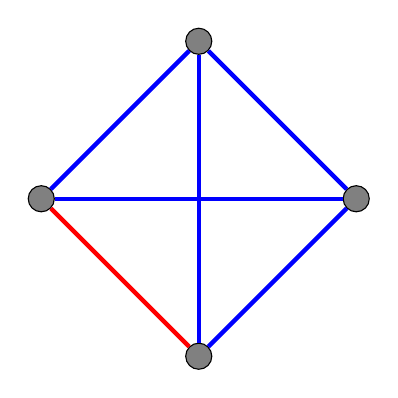
\begin{tikzpicture}[node distance={15mm}, main/.style = {draw, circle, fill = gray}] 
 \node[main] (1) at (0:2) {};
 \node[main] (2) at (90:2) {};
 \node[main] (3) at (180:2) {};
 \node[main] (4) at (270:2) {};


\draw[ultra thick][blue] (1) -- (2);
\draw[ultra thick][blue] (1) -- (3);
\draw[ultra thick][blue] (1) -- (4);
\draw[ultra thick][blue] (2) -- (3);
\draw[ultra thick][blue] (2) -- (4);
\draw[ultra thick][red] (3) -- (4);

    \end{tikzpicture}
    }
        \hspace{15mm}
        \subfloat[]{
       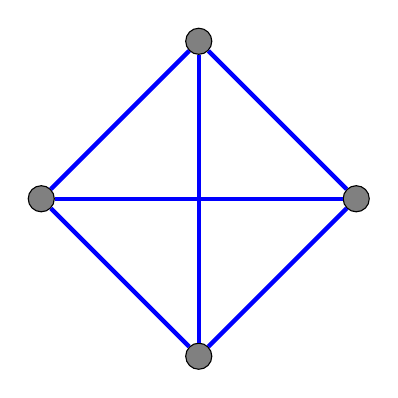
\begin{tikzpicture}[node distance={15mm}, main/.style = {draw, circle, fill = gray}] 
 \node[main] (1) at (0:2) {};
 \node[main] (2) at (90:2) {};
 \node[main] (3) at (180:2) {};
 \node[main] (4) at (270:2) {};


\draw[ultra thick][blue] (1) -- (2);
\draw[ultra thick][blue] (1) -- (3);
\draw[ultra thick][blue] (1) -- (4);
\draw[ultra thick][blue] (2) -- (3);
\draw[ultra thick][blue] (2) -- (4);
\draw[ultra thick][blue] (3) -- (4);
    \end{tikzpicture}
    }
    \caption{Przykłady grafów niespełniających $R(2,4,4)$}
    \label{grafk2}
 \end{figure}
  	


  
 \hfill \par
%  \item R(3,3)=6 \hfill \par
 Rozważmy R(3,3)=6 . R(3,3) jest pierwszym nietrywialnym przykładem liczby Ramseya, lecz nadal na tyle prostym aby łatwo móc ją wyznaczyć. Łatwo można wykluczyć $\mathit{K}_{3}$, $\mathit{K}_{4}$ oraz $\mathit{K}_{5}$ za pomocą następującego pokolorowania krawędzi (rysunek \ref{grafk5}).


\begin{figure}[H]
  \centering
   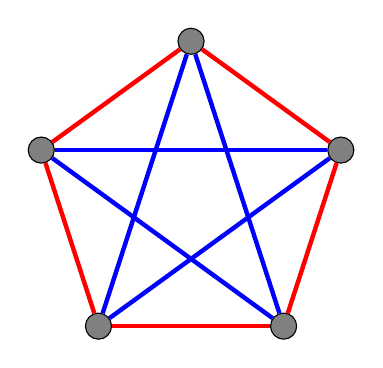
\begin{tikzpicture}[node distance={15mm}, main/.style = {draw, circle, fill = gray}] 
 \node[main] (1) at (1*90:2) {};
 \node[main] (5) at (1*162:2) {};
 \node[main] (4) at (1*234:2) {};
 \node[main] (3) at (1*306:2) {};
 \node[main] (2) at (1*18:2) {};

\draw[ultra thick][red] (1) -- (2);
\draw[ultra thick][red] (2) -- (3);
\draw[ultra thick][red] (3) -- (4);
\draw[ultra thick][red] (4) -- (5);
\draw[ultra thick][red] (5) -- (1);

\draw[ultra thick][blue] (1) -- (3);
\draw[ultra thick][blue] (1) -- (4);
\draw[ultra thick][blue] (2) -- (4);
\draw[ultra thick][blue] (2) -- (5);
\draw[ultra thick][blue] (3) -- (5);
    \end{tikzpicture}
    \caption{Graf $R(3,3,5)$}
    \label{grafk5}
 \end{figure}

Powyższy rysunek pokazuje sposób kolorowania dla grafu 5-wierzchołkowego, ale wykluczenie dowolnego wierzchołka daje poprawne kolorowanie dla grafu 4-wierzchołkowego, dowolnych dwóch dla grafu 3-wierzchołkowego itd.

Aby udowodnić że $R(3,3) = 6$ przeanalizujmy kolorowanie grafu pełnego o 6 wierzchołkach. 


\begin{figure}[H]
  \centering
  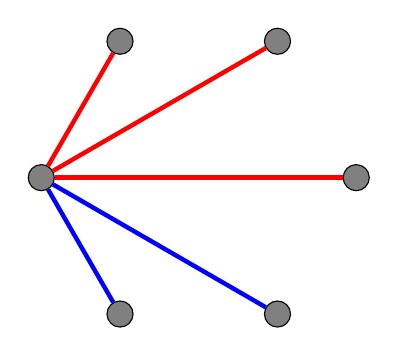
\begin{tikzpicture}[node distance={15mm}, main/.style = {draw, circle, fill = gray}] 
 \node[main] (3) at (0:2) {};
 \node[main] (2) at (60:2) {};
 \node[main] (1) at (120:2) {};
 \node[main] (6) at (180:2) {};
 \node[main] (5) at (240:2) {};
 \node[main] (4) at (300:2) {};

\draw[ultra thick][red] (6) -- (1);
\draw[ultra thick][red] (6) -- (2);
\draw[ultra thick][red] (6) -- (3);
\draw[ultra thick][blue] (6) -- (4);
\draw[ultra thick][blue] (6) -- (5);
    \end{tikzpicture}
    \caption{Pokolorowane krawędzie wychodzące z jednego wieszchołka}
    \label{graf61}
 \end{figure}

 \begin{figure}[H]
  \centering
  \subfloat[]{
   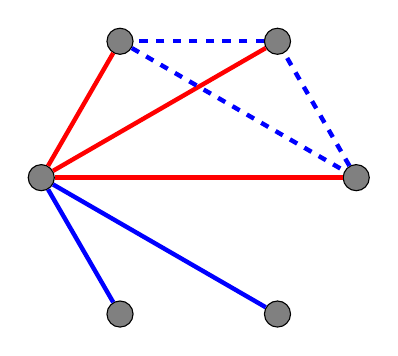
\begin{tikzpicture}[node distance={15mm}, main/.style = {draw, circle, fill = gray}]  
 \node[main] (3) at (0:2) {};
 \node[main] (2) at (60:2) {};
 \node[main] (1) at (120:2) {};
 \node[main] (6) at (180:2) {};
 \node[main] (5) at (240:2) {};
 \node[main] (4) at (300:2) {};

\draw[ultra thick][red] (6) -- (1);
\draw[ultra thick][red] (6) -- (2);
\draw[ultra thick][red] (6) -- (3);
\draw[ultra thick][blue] (6) -- (4);
\draw[ultra thick][blue] (6) -- (5);

\draw[ultra thick][blue, dashed] (2) -- (1);
\draw[ultra thick][blue, dashed] (3) -- (2);
\draw[ultra thick][blue, dashed] (1) -- (3);
    \end{tikzpicture}
    }
 \hspace{15mm}
 \subfloat[]{
      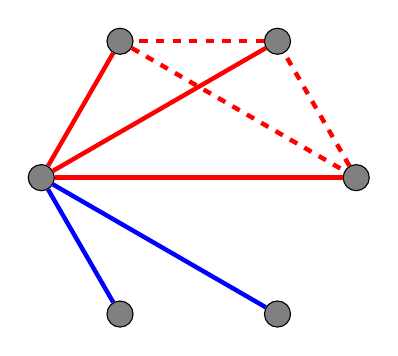
\begin{tikzpicture}[node distance={15mm}, main/.style = {draw, circle, fill = gray}] 
 \node[main] (3) at (0:2) {};
 \node[main] (2) at (60:2) {};
 \node[main] (1) at (120:2) {};
 \node[main] (6) at (180:2) {};
 \node[main] (5) at (240:2) {};
 \node[main] (4) at (300:2) {};

\draw[ultra thick][red] (6) -- (1);
\draw[ultra thick][red] (6) -- (2);
\draw[ultra thick][red] (6) -- (3);
\draw[ultra thick][blue] (6) -- (4);
\draw[ultra thick][blue] (6) -- (5);

\draw[ultra thick][red, dashed] (2) -- (1);
\draw[ultra thick][red, dashed] (3) -- (2);
\draw[ultra thick][red, dashed] (1) -- (3);
    \end{tikzpicture}
    }
    \caption{Pokolorowania implikujące powstanie czerwonej lub niebieskiej $K_3$}
    \label{graf62}
 \end{figure}



Po wybraniu dowolnego wierzchołka i pokolorowaniu wychodzących z niego krawędzi co najmniej trzy z nich będą miały wspólny kolor. Na rysunku \ref{graf61} tym kolorem jest kolor czerwony, krawędzie tego koloru połączone są z trzema innymi wierzchołkami. Patrząc na trzy wierzchołki do których zostały poprowadzone krawędzie czerwone, łatwo zauważyć, że aby uniknąć powstania trójkąta czerwonego należy połączyć te wierzchołki kolorem niebieskim, lecz robiąc to powstanie klika o rozmiarze trzy koloru niebieskiego (rysunku \ref{graf62}). Dowodzi to że $R(3,3) = 6$.
    

\hfill \par

%\item Inne liczby Ramseya \hfill \par

 Udowodnienie wartości pozostałych liczb Ramseya zostanie pominięte, gdyż: stopień skomplikowania dowodu rośnie wraz z ilością wierzchołków, nie istnieje żaden znany łatwy obliczeniowo sposób na określenie dokładnej wartości tej liczby, oraz wyznaczenie dokładnej wartości często jest na tyle trudne że istnieje jedynie jej bliższe oszacowanie. Tabela \ref{tabwartosci} prezentuje dokładne wartości, lub górne i dolne ograniczenie dla dwukolorowych liczb Ramseya $R(k,l)$ $k<10$, $l<10$ (wartości dla $k$ i $l$ równego 2 albo 1 zostały opisane wcześniej). Jako że wartości dla liczb Ramseya są symetryczne ($R(r,b)$ = $R(b,r)$) wypełniony został jedynie górny trójkąt w tabeli.
 
\begin{table}[H]
  \centering
%
\begin{tabular}{|p{0.9cm}|p{0.9cm}|p{0.9cm}|p{0.9cm}|p{0.9cm}|p{0.9cm}|p{0.9cm}|p{0.9cm}|p{0.9cm}|}
\hline
$R(k,l)$ & 3 & 4  & 5                                               & 6                                                 & 7                                                 & 8                                                  & 9                                                  & 10                                                  \\ \hline
3                  & 6 & 9  & 14                                              & 18                                                & 23                                                & 28                                                 & 36                                                 & \begin{tabular}[c]{@{}l@{}}40\\ 42\end{tabular}     \\ \hline
4                  &   & 18 & 25                                              & \begin{tabular}[c]{@{}l@{}}36\\ 41\end{tabular}   & \begin{tabular}[c]{@{}l@{}}49\\ 61\end{tabular}   & \begin{tabular}[c]{@{}l@{}}59\\ 84\end{tabular}    & \begin{tabular}[c]{@{}l@{}}73\\ 115\end{tabular}   & \begin{tabular}[c]{@{}l@{}}92\\ 149\end{tabular}    \\ \hline
5                  &   &    & \begin{tabular}[c]{@{}l@{}}43\\ 49\end{tabular} & \begin{tabular}[c]{@{}l@{}}58\\ 87\end{tabular}   & \begin{tabular}[c]{@{}l@{}}80\\ 143\end{tabular}  & \begin{tabular}[c]{@{}l@{}}101\\ 216\end{tabular}  & \begin{tabular}[c]{@{}l@{}}133\\ 316\end{tabular}  & \begin{tabular}[c]{@{}l@{}}143\\ 442\end{tabular}   \\ \hline
6                  &   &    &                                                 & \begin{tabular}[c]{@{}l@{}}102\\ 165\end{tabular} & \begin{tabular}[c]{@{}l@{}}115\\ 298\end{tabular} & \begin{tabular}[c]{@{}l@{}}134\\ 495\end{tabular}  & \begin{tabular}[c]{@{}l@{}}183\\ 780\end{tabular}  & \begin{tabular}[c]{@{}l@{}}204\\ 1171\end{tabular}  \\ \hline
7                  &   &    &                                                 &                                                   & \begin{tabular}[c]{@{}l@{}}205\\ 540\end{tabular} & \begin{tabular}[c]{@{}l@{}}217\\ 1031\end{tabular} & \begin{tabular}[c]{@{}l@{}}252\\ 1713\end{tabular} & \begin{tabular}[c]{@{}l@{}}292\\ 2826\end{tabular}  \\ \hline
8                  &   &    &                                                 &                                                   &                                                   & \begin{tabular}[c]{@{}l@{}}282\\ 1870\end{tabular} & \begin{tabular}[c]{@{}l@{}}329\\ 3583\end{tabular} & \begin{tabular}[c]{@{}l@{}}343\\ 6090\end{tabular}  \\ \hline
9                  &   &    &                                                 &                                                   &                                                   &                                                    & \begin{tabular}[c]{@{}l@{}}565\\ 6588\end{tabular} & \begin{tabular}[c]{@{}l@{}}581\\ 12677\end{tabular} \\ \hline
10                 &   &    &                                                 &                                                   &                                                   &                                                    &                                                    & \begin{tabular}[c]{@{}l@{}}798\\ 23556\end{tabular} \\ \hline
\end{tabular}%

 \caption{Wartości liczb ramseya dla 3$\leq$k$\leq$10 i 3$\leq$l$\leq$10. Górny wiersz odpowiada wartościom $k$ a boczny wartościom $l$. Dwie liczby zapisane w jednej komórce oznaczają ograniczenie dla danej liczby: najpierw zapisana jest dolne a następnie górne ograniczenie}
 \label{tabwartosci}
\end{table}
\hfill 


Istnieją dwa główne podejścia na wyznaczanie liczb Ramseya. Pierwszym z nich, gdy wyznaczenie dokładnej liczby nie jest możliwe polega na wyznaczeniu górnego oraz dolnego ograniczenia. Przykładową pracą gdzie udowadniane było ograniczenie dla liczb Ramseya ($R(5,5) \leq 49$ oraz $R(4,6) \leq 41$) jest praca Brendana D. McKaya oraz Stanisława P. Radziszowskiego ''Subgraph Counting Identities and Ramsey Numbers'' \cite{boundproof}. Drugim sposobem natomiast jest wyznaczenie dokładnej wartości tej liczby. W tym przypadku bardzo często wykorzystywane są komputery z zaprojektowanymi do tego celu algorytmami. Przykładowymi pracami gdzie ta metoda została wykorzystana jest praca na której bazujemy, autorstwa Brendana D. McKaya oraz Stanisława P. Radziszowskiego $R(4,5)=25$\cite{mainpaper} oraz praca Charlesa M. Grinsteada i Sama M. Robertsa ''On the Ramsey Numbers R(3,8) and R(3,9)'' gdzie posłużyli się algorytmem do wyznaczenia $R(3,9)=36$ oraz ustalenia ograniczenia dla liczby $R(3,8)$ ($28 \leq R(3,8) \leq 29$)\cite{computeproof}. \par

Powodem dla podawania dolnego oraz górnego ograniczenia jest, jak wspomniano wcześniej, brak uniwersalnej i opłacalnej formuły do określenia dokładnej wartości. Dla grafu pełnego $\mathit{K}_{n}$, który ma ${\dfrac{n(n-1)}{2}}$ krawędzi, istnieje $c^{\dfrac{n(n-1)}{2}}$ grafów które trzeba przeszukać (gdzie $c$ oznacza liczbę kolorów). Oznacza to że złożoność przeszukiwania wszystkich możliwych grafów metoda naiwną to $O(c^{n^{2}})$ przy $c$ kolorach i $n$ wierzchołkach. Przykładowo dla $R(4,6)$ gdybyśmy chcieli sprawdzić dolną granicę 36 \cite{smallramsey}, należałoby sprawdzić wszystkie dwukolorowania $\mathit{K}_{36}$, który ma ${36\choose 2}$ = 630 krawędzi. Istnieje więc $2^{630} \approx 4,4555 \cdot 10^{189}$ różnych sposobów na pokolorowanie tego grafu. Dlatego przy obecnych możliwościach obliczeniowych nie jest możliwe rozwiązanie tego problemu używając podejścia naiwnego. \par

Aby podsumować problem znajdowania dokładnych warości liczb Ramseya można posłużyć się słowami Paula Erdősa: Jeżeli kosmici najechaliby ziemię i postawili ultimatum, że jeżeli ludzkość nie znajdzie $R(5,5)$ w ciągu roku, to zniszczą ziemię, najlepszym wyborem byłoby zebranie całej mocy obliczeniowej jaką aktualnie dysponuje ludzkość w celu pozyskania tej liczby. Jednak w przypadku gdy kosmici zażądali by R(6,6) najlepszym wyborem było by wypowiedzenie im wojny.\cite{aliens}  \par

\hfill \par
%\item Ograniczenia liczby Ramseya \hfill \par

Górne ograniczenie może być łatwo wyliczona stosując nierówność $R(r,b) \le R(r-1,b)+R(r,b-1)$ \cite{graniceupdown}. Nie jest to jednak zadowalający wynik, ani zadowalający sposób na wyznaczanie górnego limitu. Poprzednie wartości liczb Ramseya mogą nie być znane oraz samo ograniczenie przy znanych wcześniejszych wartościach nie jest najbardziej optymalną. Wzór jawny który opisuje wcześniej podany przypadek to: $R(r,b) \le {r+b-2\choose r-1}$. Przytoczone górne ograniczenie jest ograniczeniem naiwnym. Ograniczenie dolne jest wyznaczane z użyciem metod probabilistycznych. Paul Erdős jako pierwszy w 1947 roku zaprezentował dowód z użyciem metod probabilistycznych na ograniczenie dolne dla liczb $R(k,k)$\cite{erdogranica, theory}. Metoda ta opierała się na wykazaniu że w losowo pokolorowanym grafie $\mathit{K}_{n}$ prawdopodobieństwo znalezienia jednokolorowego grafu $\mathit{K}_{k}$ jest mniejsze od 1 dla pewnej wartości.

%\end{enumerate}

